\documentclass[oribibl]{llncs}
\usepackage{graphicx}
\usepackage{amsmath}

\title{Collabot}
\subtitle{A Collaborative Robotic Agent for the CiberRato Competition  }
\author{Pedro Pontes \and Tiago Varela}
\institute{Faculdade de Engenharia da Universidade do Porto}

%
\begin{document}
\maketitle
\begin{abstract}
This paper discusses the implementation of the navigation and target localization strategies for a  collaborative robotic agent using the Ciber-Rato Simulation Tools. Nevertheless, communication and mapping strategies were also implemented in the discussed agent, however those implementations are further explained in the paper \cite{baboehelder}.
To this end, we particularly focus on developing an interesting solution for a maze solver agent and explore the collaboration between robots with similar architectures.
\end{abstract}

\section{Introduction}
Ciber-Rato is a modality of the Micro-Rato contest from University of Aveiro. This modality is a competition between small autonomous robots trying to solve mazes. \cite{Lau2002} 
In this project, we faced the challenge of developing a collaborative robotic agent architecture using the Simulation Tools created for the Ciber-Rato competition. The agents should be able to solve simple mazes by finding a beacon and returning to his original position, while avoiding obstacles, collisions and dealing with time constraints. Furthermore, in the collaborative competition, the agents are playing in a team of 5 robots, all the robots, must meet in the target area, and after that return to their original position. The maze is only considered solved when all the mice return to their original position.

At the starting point, the agents have no previous information about the world state, namely the target position, maze's topology and even his or other mice positions. Therefore, a simple reactive robot architecture was not suitable for this problem and so proper communication, mapping, navigation and target localization strategies were be developed in order to maximize the agent efficiency.

In this paper, first we present the simulation system architecture. Then the agent architecture and design are analyzed, mainly focusing in the navigation and target localization strategies, since communication and mapping strategies are further discussed in the paper \cite{baboehelder}. After that, the results of the developed strategies are discussed. Finally, in the last section, are presented the main conclusions and some possible future developments.

\section{Simulation System Architecture}
To develop this project the Ciber-Rato Simulation Tools, 2012 edition, were chosen as a simulation platform. This platform allows the developers to focus only on the development of an efficient agent algorithm, eliminating the problems and challenges associated with real robots construction by providing a simulation environment that models all the hardware components of the robots and a allows the developed algorithms to be tested\cite{Lau2002}. 

The simulation environment is composed by a Simulator, a Simulation Viewer and Virtual Robots. The first is responsible for modelling all the hardware components of the robots, the maze and ensure that all the execution rules are applied. The Simulation Viewer displays the maze, the robots movements and the remaining execution time. The virtual Robots are detailed in the section bellow.

All the specifications presents in this paper are based on the Ciber-Rato 2011 Rules and Technical Specifications \cite{DepartamentodeElectronica2011}, and only a brief specification is present in here, for a more detailed specification please consult the document mentioned above.

\subsection{Virtual Robots}
The virtual robots have circular bodies and are equipped with sensors, actuators and command buttons. Only the robots' sensors and actuators used by the agent that we developed are mentioned in this section.

\subsubsection{Sensors}\hfill \\
For the developed agent the following sensors were used, from the ones available in the simulation environment: 
\begin{itemize}
  \item[\textbf{Obstacle Sensors}]
  4 proximity sensors, 3 oriented to the front of the robot (left, middle and right sides), and one in the rear. Each sensor has a 60º aperture angle.
  \item[\textbf{Beacon Sensor}]
  Measures the angular position of the beacon with respect to the robot's frontal axis. The measure ranges from −180 to +180 degrees, with a resolution of 1 degree.
  \item[\textbf{Bumper}]Active when the robot collides.
  \item[\textbf{Ground Sensor}]
  Active when the robot is completely in target area.
  \item[\textbf{Compass}]
  Positioned in the center of the robot and measures its angular position with respect to
the virtual North (X axis).
  \item[\textbf{GPS}]
  Returns the position of the robot in the arena, with resolution 0.1. It is located in the center of the robot.
\end{itemize}

\subsubsection{Actuators}\hfill \\
The actuators components of the robots used in this project are 2 motors and 1 signaling LED. 
\begin{itemize}
  \item[\textbf{Motors}]
Motors have inertia and noise in order to more closely represent real motors, and the translation or rotation movements can be achieved by applying different power values to each motor.
  \item[\textbf{LED}]
The LED is used to signal that the robot has already found the beacon.
\end{itemize}

\subsubsection{Buttons}\hfill \\
Two buttons, named Start and Stop, are provided in each robot and are used by the simulator to start and interrupt the competition.

\subsection{Arena}
The arena is randomly positioned in the world, which means that the starting coordinates of the robot may differ for every attempt to solve the maze, and has a maximum size of 14x28 um.
The arena is populated with obstacles, a target area, and a starting grid. For the same maze different starting grids can also be used. The obstacles within the arena can be higher then the beacon, making it invisible for the beacon sensor.

\subsection{Communication}
Communication between robots can be made by sending appropriate commands, through the simulator. The other agents will be then responsible for reading the messages in the simulator. However the following constraints are be applied:
\begin{itemize}
 \item Per cycle, a robot can send (broadcast) up to 100 bytes;
 \item Per cycle, a robot can read up to 400 bytes;
 \item Per cycle, a robot can read up to 400 bytes;
 \item Robots can only read messages sent from a maximum of 8 units from its current position;
 \item Obstacles do not interfere with communication;
 \item Latency of 1 cycle for sent messages.
 \end{itemize} 

\section{Agent Architecture}
In this project we faced the challenge of creating a team of 5 robotic agents, playing simultaneously, in the environment provided by the Ciber-Rato Simulation Tools. The Mice have two specific goals: locate the target area and place all the agents inside that area;return all the robots back to their original position.

In order to achieve that goal our agents must be able to fully operate in an unstructured environment by avoiding obstacles and finding the beacon in a simple to moderately complex map.However, at the starting point, the agents have no previous information about the world state, namely the target position, maze's topology and even his or other mice positions. Therefore, a simple reactive robot architecture was not suitable for this problem and so proper communication, mapping, navigation and target localization strategies were be developed in order to maximize the agents efficiency.

The developed agent architecture is composed by 6 different modules and is represented in figure 1.

\begin{figure}
  \centering
  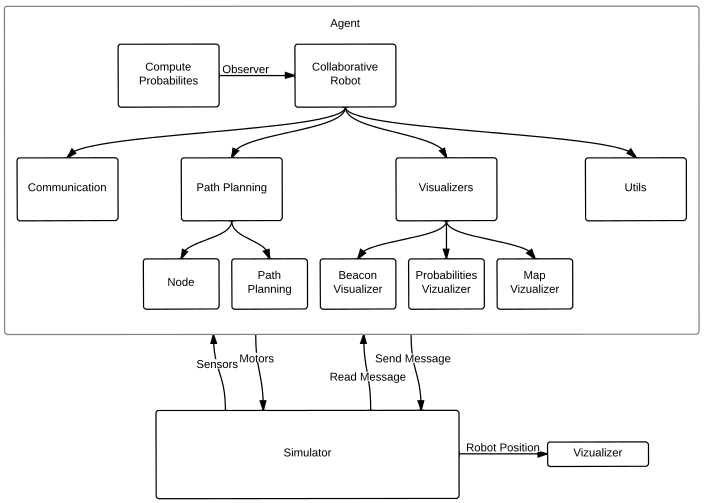
\includegraphics[width=0.9\textwidth]{robot-architecture.png}
  \label{fig:layered}
  \caption{System architecture.}
\end{figure}

Bellow, the description of each module:

\begin{itemize}
  \item[\textbf{Compute Probabilities}]
  lorem ipsum
  \item[\textbf{Communication}]
  lorem ipsum
  \item[\textbf{Path Planning}]
  lorem ipsum
  \item[\textbf{Visualizers}]
  lorem ipsum
  \item[\textbf{Utils}]
  lorem ipsum
\end{itemize}

\subsection{Navigation Strategy}
The navigation strategy followed by our robot can be divided in two fundamental steps: exploring the map before finding and reaching the beacon and returning home after finding it.

\subsubsection{Exploring the Map}

For the first phase of navigation the behavior of our mouse was mostly imported from a previously created solution of a purely reactive mouse described in \cite{Moreira2012}. This solution was inspired by the subsumption layered model that Brooks proposed for mobile robot control system\cite{Brooks_1986}, and can be viewed on figure 2.

\begin{figure}
  \centering
  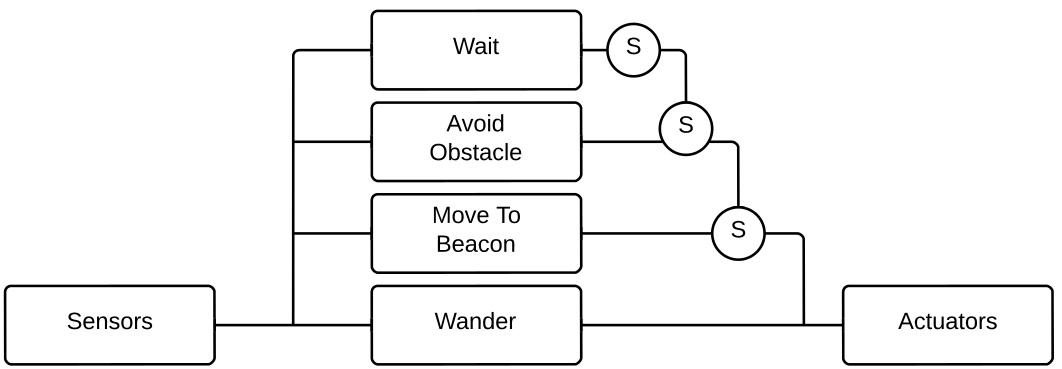
\includegraphics[width=0.8\textwidth]{layer-architecture.png}
  \label{fig:layered}
  \caption{Layered architecture.}
\end{figure}

With this system architecture the top layers are activated when certain conditions are detected by the sensors, overriding the actions of the bottom layers, e.g. if an obstacle is detected the robot will start its obstacle avoidance routine, instead of moving towards the beacon or wandering around. 

Each of these layers will now be described in further detail:
\begin{description}
  \item[\textbf{Wait}]
  This layer is used to detect if the robot has reached the beacon location and to stop its motion, also signaling to the simulator that the robot has finished the first phase of the competition.
  \item[\textbf{Avoid Obstacle}]
  In order to avoid obstacles a wall following algorithm was implemented. The mouse moves always in a clockwise direction and the strategy is held until the beacon is framed within 20º degrees of the robot.
  
  One example of a complex obstacle that can be avoided by this algorithm is represented in figure 3. At first, the robot is moving forward. When a wall is detected in front of the robot, it turns about 90º to the right, and keeps moving forward. On every inner corner,  C, the mechanism is similar to the previously described. On every outer corner, E, the robot deviates itself in order to turn and move forward without touching the corner. When the robot is rotating, it verifies if the beacon is visible within a 20º amplitude, and if that is the case the wall following is aborted and the robot moves in the direction of the beacon.
  
  \item[\textbf{Move to Beacon}]
  This layer detects if the beacon is visible and if it is the robot rotates itself to align with the beacon direction and then moves forward. This rotation value is calculated accordingly to beacon sensor information, e.g. if the beacon direction is opposite to the robot's facing direction then the rotation value is higher than if the beacon direction was only to the left or to the right of the robot.
  \item[\textbf{Wander}]
  This layer provides the default action which is for the robot to move forward, veering to the left or to the right every 100 iterations, creating an undulatory locomotion similar to that of a snake.
\end{description}

\subsubsection{Return Home}

\subsection{Path Planning}

The path planing problem in the developed solution consists in finding the best possible path between the beacon area and the original position of the robot, considering the information about the world that the robot gathered until that moment. In order to solve this problem Collabot implements an A* algorithm[] in the Path Planning module. The A* algorithm uses a best-first search based on an heuristic to find the path with the lower cost between the initial and goal points in a map.

The Path Planning module is composed by two classes, Node and PathFinder, and it implementation is not coupled to the robotic agent implementation, meaning that this module could be used to solve any problem requiring the shortest path between two points in a two dimensional matrix of doubles. Each cell of the the matrix encapsulates the cost of traveling through that cell, however if the value of a cell is higher than a preset value, the cell is considered to have an obstacle and so is not traversable. Furthermore, all the surrounding cells of a cell are considered as a neighbor, therefore in best possible situation a cell can have 8 neighbors. A cell that is not traversable is not considered as a neighbor of any cell.

To find the best possible path between two points the A* uses an heuristic function to determine the order in which nodes are visited during the search for that path. Equation 1 defines the cost function \textit{f(x)} as the sum of the distance so far traveled, \textit{g(x)}, and the estimated distance to the target, \textit{h(x)}. The estimated distance to the target, represented in equation 2, is computed using the euclidean distance[] between the current point, \textit{p}, and the goal point, \textit{q}, and returns the length of the line segment connecting the two points.

\begin{equation}
f(x) = g(x) + h(x)
\end{equation}

\begin{equation}
h(x) = \sqrt{(p_x - q_x)^2 + (p_y - q_y)^2}
\end{equation}

Finally, in order to ensure that is always possible to travel through the calculated path without touching the walls, the implemented solution also allows the enlargement of the walls of the the maze in the size of the robot radius. To do so, for every node, \textit{N}, of the provided matrix that is not traversable and has not been visited yet, the surroundings nodes, are calculated and the node \textit{N} is marked as visited. If the cost of a surrounding node, \textit{S}, is smaller then the cost of the current node \textit{N}, the cost of \textit{S} is updated to the cost of \textit{N} and \textit{S} is marked as visited.





\subsection{Target Localization}
lorem ipsum

\section{Results}
lorem ipsum
----------------- old description -------------------------
\subsection{Limitations and Benefits}
This reactive architecture includes some limitations, such as:

\begin{itemize}
  \item if the robot is following the beacon and there is an concave obstacle in the way, most of the times, the robot will be stuck around the same place with conflicting orders to follow the beacon and to avoid the obstacle in front. The rule to only follow the beacon on every 50 iterations was developed to try to circumvent this cases and provided promising results;
  \item by not being able to store the world state the robot wanders around the map without knowing if it has already been there, and this can also create cycles, specially if the robot is surrounded by walls and there is only one way out.
\end{itemize}

The benefits of this type of architecture are that the robot is able to quickly react to dynamic changes in the environment, such as the introduction of a new robot in the system, and also able to react to some environment variable that the robot's programmer has not foreseen.

----------------- end of old description -------------------------


\section{Conclusion}
lorem ipsum

\section{Future Work}
lorem ipsum
\bibliography{report}
\bibliographystyle{splncs}
\end{document}